% Requires graphicx (already loaded in the manuscript).
\begin{figure*}[t]
    \centering
    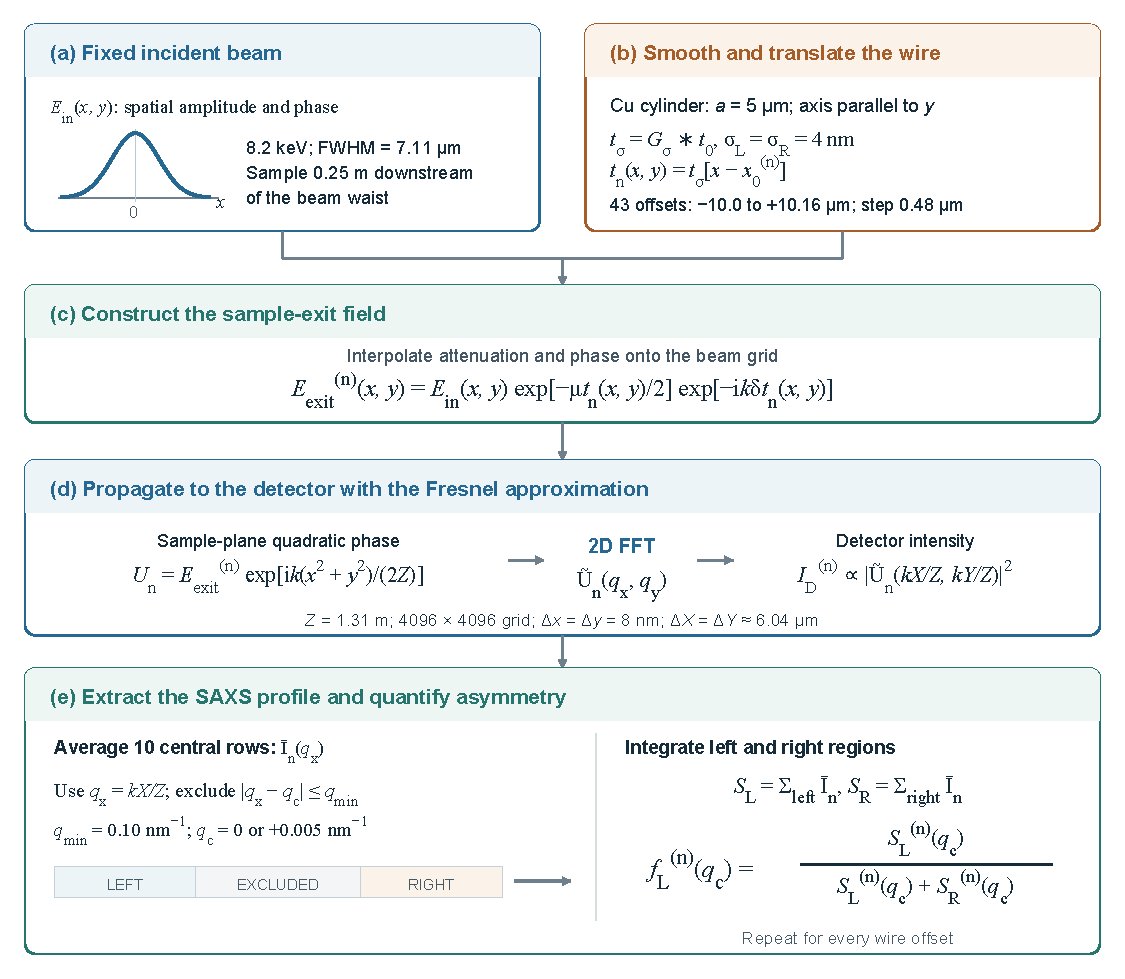
\includegraphics[width=0.96\textwidth]{03_saxs_workflow.pdf}
    \caption{Workflow for the SAXS simulation and asymmetry analysis. The fixed incident field and the Gaussian-smoothed, translated wire thickness are combined to form the sample-exit field. Fresnel propagation is evaluated by applying the sample-plane quadratic phase, performing a two-dimensional Fourier transform, and taking the squared magnitude of the propagated field. The ten central detector rows are averaged to obtain a one-dimensional SAXS profile. Left and right intensity sums are evaluated outside a central exclusion window for $q_c=0$ and $q_c=+0.005\,\mathrm{nm}^{-1}$, and the left-side fraction $f_L$ is calculated at each wire offset. The Gaussian icon is schematic; the colored strip denotes integration regions.}
    \label{fig:saxs_workflow}
\end{figure*}
